\item A barra uniforme de \SI{50}{\kilogram} está em repouso em uma posição vertical quando a corda fixada a ela em $B$ é submetida a uma força $P=\SI{250}{\newton}$. Determine a aceleração angular inicial da barra e a intensidade da força reativa que o pino $A$ exerce sobre a roda. Despreze a dimensão do pino liso em $C$.


\vspace{-.6cm}
\begin{flushright}
	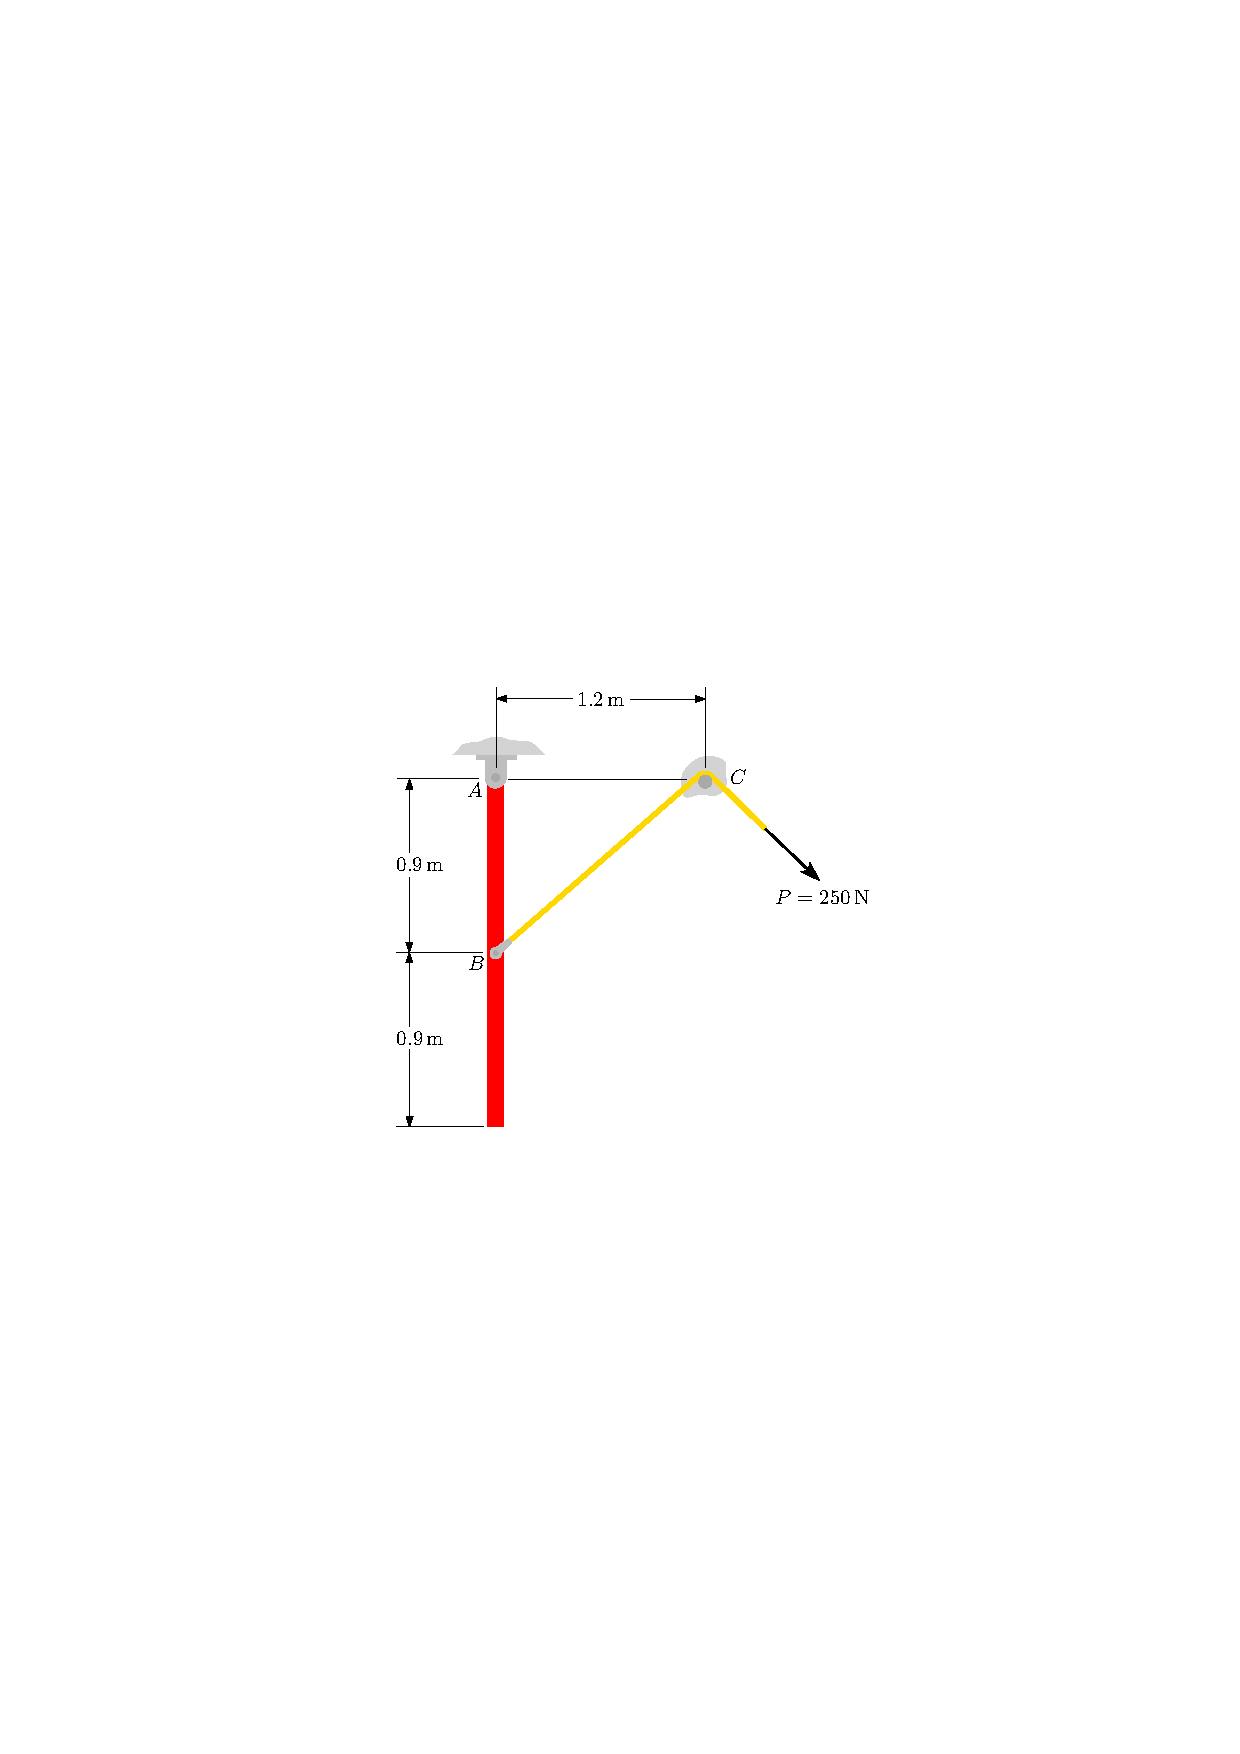
\includegraphics[scale=1.2]{../../images/draw_8}
\end{flushright}